\documentclass[acmtog,nonacm]{acmart}

%% Changelog
% Referenzen eingedeutscht (Fig. zu Abbildung, Table zu Tabelle) Anführungszeichen eingedeutscht
% Wissentschaftliche Schreibweise überprüfen und ggfs. einführen
% Referenz von Tanenbaum und Bos in Abschnitt 6 geändert
% Typo in Autorenname korrigiert (Nocholas zu Nicholas)
% unnötige erwähnungen von zb slift weglassen
% Magische Werte besser erläutern
% Formel zur Berechnung der Adresse im Shadow Memory nummeriert
% Tausch der Satzreihenfolge bei der Erklärung zu Speicherfehlerarten


%% Packages
%% Use german language
\usepackage[ngerman]{babel}
%% Add code listings to text
\usepackage{listings}
%% Use graphics
%%\usepackage[ngerman]{graphicx}
%% Outline
\usepackage{outlines}
%% Better referencing
\usepackage[capitalise,ngerman]{cleveref}
%% Colors in tables
\usepackage[table,xcdraw]{xcolor}
%% Configure captions
\usepackage{caption} 
\captionsetup[figure]{name=Abb.}
\usepackage{bibgerm}

\definecolor{codegreen}{rgb}{0,0.6,0}
\definecolor{codegray}{rgb}{0.5,0.5,0.5}
\definecolor{codepurple}{rgb}{0.58,0,0.82}
\definecolor{backcolour}{rgb}{0.95,0.95,0.92}


\lstdefinestyle{mystyle}{
  %backgroundcolor=\color{backcolour},
  commentstyle=\color{codegreen},
  keywordstyle=\color{magenta},
  numberstyle=\tiny\color{codegray},
  stringstyle=\color{codepurple},
  basicstyle=\ttfamily,%\footnotesize,
  breakatwhitespace=false,
  breaklines=true,
  captionpos=b,
  keepspaces=true,
  numbers=left,
  numbersep=5pt,
  showspaces=false,
  showstringspaces=false,
  showtabs=false,
  tabsize=2
}

\lstset{style=mystyle}

\AtBeginDocument{%
  \providecommand\BibTeX{{%
    Bib\TeX}}}

\citestyle{acmnumeric}

\begin{document}

\title{Ansätze zur automatisierten Speicherfehlererkennung}

\author{Florian Dinter}
\email{florian.dinter@student.uni-siegen.de}
\affiliation{%
  \institution{Universität Siegen}
  \city{Siegen}
  \state{Nordrhein Westfalen}
  \country{Deutschland}
}

%%\renewcommand{\shortauthors}{Florian Dinter}

%% TODO: Text etwas umschreiben -> kommt von ChatGpt
\begin{abstract}
  Speicherzugriffsfehler, wie beispielsweise Out-of-Bounds-Zugriffe
  und die Nutzung bereits freigegebenen Speichers, stellen nach wie
  vor ein gravierendes Problem für Programmiersprachen wie C und C++
  dar. Dieses Paper fasst zwei bedeutende Ansätze zur Erkennung von
  Speicherfehlern zusammen und vergleicht deren Wirksamkeit und
  Leistung: den neu entwickelten "`mcds"'und den etablierten AddressSanitizer.
\end{abstract}

\begin{CCSXML}
  <ccs2012>
  <concept>
  <concept_id>10002978.10003022.10003023</concept_id>
  <concept_desc>Security and privacy~Software security engineering</concept_desc>
  <concept_significance>100</concept_significance>
  </concept>
  </ccs2012>
\end{CCSXML}

\ccsdesc[100]{Security and privacy~Software security engineering}

\maketitle

\section{Einleitung}

Die Erkennung von Speicherzugriffsfehlern ist ein entscheidender Aspekt der
Softwareentwicklung, insbesondere für Programme, die in den unsicheren Sprachen
C und C++ geschrieben sind. Speicherzugriffsfehler wie Out-of-Bounds-Zugriffe
und die Nutzung bereits freigegebenen Speichers (Use-After-Free) können
schwerwiegende Folgen haben, darunter Programmabstürze, Datenkorruption und
Sicherheitslücken, die von Angreifenden ausgenutzt werden können. Die
Motivation zur Entwicklung effektiver Werkzeuge zur Fehlererkennung ergibt sich
aus der Notwendigkeit, diese Probleme frühzeitig zu identifizieren und zu
beheben, um die Zuverlässigkeit und Sicherheit von Software zu gewährleisten.

Die Bedeutung der Fehlererkennung von Speicherzugriffen ist weitreichend.
Speicherzugriffsfehler gehören zu den häufigsten und zugleich gefährlichsten
Fehlern in Software. Sie können zu unvorhersehbarem Verhalten führen, das
schwer zu diagnostizieren und zu beheben ist. Insbesondere in
sicherheitskritischen Anwendungen, wie z.B. Betriebssystemen, Webbrowsern und
Server-Software, ist die präzise Erkennung und Beseitigung solcher Fehler
unerlässlich, um Angriffe zu verhindern und die Integrität der Systeme zu
bewahren.

Die Relevanz dieser Thematik ist besonders für die Programmiersprachen C und
C++ von hoher Bedeutung. Diese Sprachen bieten aufgrund ihrer
Leistungsfähigkeit und Flexibilität direkten Zugriff auf Speicher, was für
viele Anwendungen vorteilhaft ist. Gleichzeitig erhöht dieser direkte Zugriff
jedoch das Risiko von Speicherfehlern, da die Programmierenden selbst für die
Speicherverwaltung verantwortlich sind. Im Gegensatz zu Sprachen mit
automatischer Speicherverwaltung, wie Java oder Python, bieten C und C++ keine
eingebauten Mechanismen zur Vermeidung von Speicherzugriffsfehlern. Daher ist
die Entwicklung leistungsfähiger Werkzeuge zur Erkennung und Behebung solcher
Fehler in C und C++ besonders wichtig.

Die vorliegende Arbeit untersucht zwei bedeutende Werkzeuge zur Erkennung von
Speicherzugriffsfehlern: den neu entwickelten "`mcds"' und den etablierten
AddressSanitizer. Beide Ansätze zielen darauf ab, Speicherzugriffsfehler
in Programmen zu identifizieren und zu beheben, um die Zuverlässigkeit und
Sicherheit der Software zu erhöhen.

\section{Grundlagen}\label{sec:grundlagen}

Speicherfehler sind eine der häufigsten und schwerwiegendsten Klassen von
Fehlern in Software, die in den Programmiersprachen C und C++ entwickelt wird.
Diese Fehler entstehen oft durch unsachgemäßen Umgang mit Speicher,
insbesondere aufgrund der direkten Kontrolle, die diese Sprachen über
Speicherzuweisungen und -freigaben bieten. Solche Fehler können zu
unvorhersehbarem Verhalten, Programmabstürzen, Datenkorruption und
Sicherheitslücken führen, die potenziell von Angreifenden ausgenutzt werden
können.

\subsection{Arten von Speicherfehlern}

In diesem Abschnitt erläutern wir verschiedene Arten von Speicherzugriffen, die 
häufig auftreten. Grundsätzlich lässt sich zwischen "`Spatial Memory Corruption"' und "`Temporal
Memory Corruption"' unterscheiden. Spatial Memory Corruption tritt auf, wenn
versucht wird, auf eine Speicheradresse zuzugreifen, die außerhalb der
zugewiesenen Speichergrenzen liegt. Temporal Memory Corruption tritt auf, wenn
versucht wird, auf eine Speicheradresse zuzugreifen, die bereits freigegeben
wurde oder deren Speicherobjekt nicht mehr gültig ist~\cite{mcds_2023}. Ein
häufiges Problem ist der Out-of-Bounds Access, bei dem ein Programm auf
Speicher zugreift, der außerhalb des zugewiesenen Bereichs eines Arrays oder
eines anderen Speicherobjekts liegt. Ein Out-Of-Bounds Zugriff kann zu unerwartetem Verhalten
führen, da der Speicherbereich außerhalb der Grenzen möglicherweise Daten
enthält, die für andere Teile des Programms oder des Betriebssystems relevant
sind.~\cref{lst:out-of-bounds} zeigt einen solchen Out-Of-Bounds Access. Beim
Zugriff auf den siebten Index des Arrays wird Speicher ausgelesen, der nicht im
Wertebereich des Arrays liegt. Solche Speicherzugiffe bringen somit ein unvorhersehbares Verhalten mit sich.

\lstinputlisting[caption={Out-Of-Bounds Access}, label={lst:out-of-bounds}, language=C++]{ressources/out-of-bounds-access.cpp}

Ein weiteres häufiges Problem ist der Use-After-Free-Fehler, der
in~\cref{lst:use-after-free} veranschaulicht wird. In~\cref{lst:use-after-free} wird ein Pointer erstellt, der auf einen
Integer im Speicher zeigt. Dieser Integer wird auf der Konsole ausgegeben und
anschließend gelöscht. Bei der wiederholten Ausgabe auf der Konsole sind die
Folgen unvorhersehbar, da der Speicher direkt von anderen Teilen des Programmes
oder des Betriebssystems verwendet werden kann. Use-After-Free-Fehler entstehen, wenn ein Programm auf einen Speicherbereich zugreift, der bereits
freigegeben wurde. Nachdem der Speicher freigegeben wurde, kann er vom
Betriebssystem oder von anderen Teilen des Programms für andere Zwecke
wiederverwendet werden, was zu Datenkorruption oder Programmabstürzen führen
kann. 

\lstinputlisting[caption={Use-After-Free}, label={lst:use-after-free}, language=C++]{ressources/use-after-free.cpp}

Analog zum Use-After-Free-Fehler gibt es den Write-After-Free-Fehler.~\cref{lst:write-after-free} zeigt, wie der
Speicherbereich für einen Integer allokiert wird. Anschließend wird der
Speicherbereich durch die \verb|free|-Anweisung wieder freigegeben. Nach der
Speicherfreigabe wird versucht, einen Wert zu schreiben. Write-After-Free-Fehler entstehen beim Versuch, einer Variable einen Wert zuzuweisen, deren Speicherbereich
schon freiegeben wurde.
Write-After-Free-Fehler können zu undefiniertem Verhalten führen, da der Speicher
möglicherweise anderweitig durch das Programm oder Betriebssystem verwendet
wird.

\lstinputlisting[caption={Write-After-Free}, label={lst:write-after-free}, language=C]{ressources/write-after-free.c}

Ein weiteres Problem sind Speicherlecks, die entstehen, wenn ein Programm
Speicher zuweist, diesen jedoch nicht wieder freigibt, nachdem er nicht mehr
benötigt wird. Dies kann im Laufe der Zeit zu einem übermäßigen
Speicherverbrauch führen und letztendlich dazu, dass dem System der Speicher
ausgeht.

%% Buffer Overflow

Die Auswirkungen von Speicherfehlern können vielfältig und schwerwiegend sein.
Zu den häufigsten Folgen gehören Programmabstürze, die oft mit einem
\verb|Segmentation Fault| (Speicherzugriffsverletzung) einhergehen, sowie
Datenkorruption, die die Datenintegrität beeinträchtigen kann, indem sie
unbeabsichtigt Daten überschreibt, was zu unvorhersehbarem Verhalten und
falschen Ergebnissen führt. Besonders gravierend sind die Sicherheitslücken,
die durch Speicherfehler entstehen können. Angreifende können diese Fehler
ausnutzen, um bösartigen Code auszuführen oder vertrauliche Daten zu stehlen.
Buffer Overflows und Use-After-Free-Fehler sind häufige Angriffsvektoren für
Exploits.

\subsection{Techniken zur Speicherfehlererkennung}

Aus der Notwendigkeit heraus, Speicherfehler zu erkennen und verhindern, wurden
Techniken entwickelt die diese Aufgabe übernehmen und die Programmierenden bei
ihrer Arbeit unterstützen. In diesem Kapitel erläutern wir Techniken, die auch in AddressSanitizer und "`mcds"' Anwendung finden.

\subsubsection{Shadow Memory}\label{sec:shadow-memory}

Beim Shadow Memory werden Metadaten für jede Speichereinheit der Anwendung
gespeichert. Dabei wird eine Speicheradresse der Anwendung auf eine Adresse im
\textit{Shadow Memory} abgebildet. Die Abbildung passiert je nach
Implementierung entweder durch eine direkte Skalierung und Offset oder durch
zusätzliche Übersetzungsebenen, die Gebrauch von einer Lookup-Tabelle machen.

Die Verwendung von \textit{Shadow Memory} resultiert in einen höheren
Speicherverbrauch der Anwendung beziehungsweise einer Verkleinerung des
nutzbaren Speichers innerhalb der Anwendung. TainTrace verwendet eine
direkte Abbildung des \textit{Shadow Memories} und benötigt ein \textit{Shadow
  Memory} mit derselben Größe wie der des Anwendungsspeichers. Dies kann zu
Problemen bei Anwendungen führen, die nicht mit dem halben Speicher auskommen
können~\cite{taint_trace_2006}. Im Gegensatz dazu ist der Speicherbedarf des
\textit{Shadow Memories} von LIFT nur ein Achtel des
Anwendungspeicherraums und ist damit effizienter als
TainTrace~\cite{lift_2006}.

Bei der Nutzung einer mehrstufigen Übersetzung des Anwendungsspeichers in den
\textit{Shadow Memory} werden zusätzliche Speicherzugriffe benötigt. Durch die
Verwendung von Lookup-Tabellen wird eine höhere Flexibilität des
Addresslayouts der Anwendung erreicht.

\subsubsection{Binäre Instrumentierung}\label{sec:binary-instrumentation}

Binäre Instrumentierung ist eine Technik, die verwendet wird, um zusätzliche
Anweisungen in bereits kompilierte Programme (\textit{Binaries})
einzufügen~\cite{nethercore_dynamic_2004}. Das Laufzeitverhalten eines
Programms kann so analysiert und modifiziert werden, ohne dass der Quellcode
des Programms geändert werden muss. So kann auch proprietäre und closed-source
Software instrumentiert werden. Dennoch kann binäre Instrumentierung zu einem
Laufzeit-Overhead führen, da zusätzliche Anweisung ausgeführt werden müssen.
Zusätzlich kann binäre Instrumentierung aufgrund der hohen Komplexität
fehleranfällig sein.

Man unterscheidet zwischen zwei Arten der binären Instrumentierung. Bei der
statischen binären Instrumentierung wird der Binärcode eines Programms vor
seiner Ausführung modifiziert. Das Werkzeug analysiert also den binären
Programmcode, fügt Instrumentierungscode ein und speichert das modifizierte
Programm ab. Bei der dynamischen Instrumentierung fügt das Werkzeug den
Instrumentierungscode zur Laufzeit ein. Das Einfügen zur Laufzeit ermöglicht
es, den Instrumentierungscode abhängig vom aktuellen Zustand und Verhalten des
Programms einzufügen.

Tools zu Speicherfehlererkennung nutzen binäre Instrumentierung, um eine
Vielfalt an Fehlern zu erkennen. Valgrind~\cite{valgrind_2007},
Dr. Memory~\cite{dr-memory_20011}, Purify~\cite{purify_1991},
BoundsChecker~\cite{bounds-checker_2024},
Intel Parallel Inspector~\cite{intel-inspector_2024} und
Discover~\cite{oracle-discover_2024} sind bekannte Tools, die binäre
Instrumentierung nutzen und Out-Of-Bounds, sowie Use After Free Fehler ohne
Fehlalarme (falsch positive) erkennen. Während diese Tools keine
Out-Of-Bounds-Fehler im Stack erkennen können, erkennen sie aber
uninitialisierte Lesezugriffe.

\subsubsection{Erweiterte Speicherallokatoren}\label{sec:debug-allocators}

Debug Allocators sind spezialisierte Speicherallokatoren, die verwendet werden,
um Speicherfehler wie Out-of-Bounds-Zugriffe und Use-After-Free Fehler zu
erkennen. Diese Techniken ändern nicht die Programmausführung selbst, sondern
arbeiten durch modifizierte Speicherzuweisungs- und Freigaberoutinen.

Werkzeuge, wie zum Beispiel GuardMalloc~\cite{guard-malloc_2024} nutzen einen
Speicherseiten basierten Schutz, um Speicherfehler zu erkennen. Eine
Speicherseite ist eine festgelegte Größe eines zusammenhängenden Blocks im
virtuellen Speicher, der sowohl im physischen RAM als auch im virtuellen
Adressraum des Prozesses verwendet wird. Speicherseiten sind ein zentraler
Bestandteil der Speicherverwaltung und des Paging-Mechanismus, der in modernen
Betriebssystemen verwendet wird~\cite{tanenbaum-modern_2015}.

Beim Speicherseitenschutz wird jeder Allokation von Speicher eine eigene Seite
im virtuellen Speicher zugewiesen. Zusätzliche Seiten rechts und links werden
als nicht-zugreifbar markiert. Wenn ein Programm versucht, auf diese
geschützten Seiten zuzugreifen -- zum Beispiel bei einer Out-Of-Bounds
Operation --, löst dies einen Out-Of-Bounds Fehler aus. Der Mechanismus zum
Speicherseitenschutz kann allerdings zu einem hohen Speicherverbrauch führen
und dazu noch langsam sein, was bei \verb|malloc|-intensiven Programmen
auffällt, da jeder \verb|malloc|-Aufruf mindestens einen Systemaufruf
erfordert.

Eine weitere Möglichkeit des Speicherseitenschutzes ist es, Redzones um die
Speicherregionen hinzuzufügen und mit "`magischen"' Werten zu füllen. Magische Werte bestehen aus Konstanten, die leicht wiedererkannt werden können, aber im normalen Programmfluss nicht vorkommen. Der Wiedererkennungswert der magischen Werte dient dazu, verschiedene Bereiche mit magischen Werten markieren zu können. Die \verb|free| Anweisung schreibt ebenfalls magische Werte in die betreffende
Speicherregion. Wenn ein "`magischer"' Wert gelesen wird, hat das Programm
einen Out-Of-Bounds Fehler erzeugt oder auf nicht initialisierte Werte
zugegriffen. Wird ein magischer Wert in einer Redzone überschrieben, wird dies
erst später erkannt, wenn die Redzone bei der Speicherfreigabe überprüft wird.
Das Werkzeug weiß jedoch nicht genau, wann der Out-Of-Bounds Schreibvorgang
oder Write-After-Free Fehler aufgetreten ist. Werkzeuge wie
DieHarder~\cite{die-harder_2010} machen sich diese Technik zu Nutze.

\subsubsection{Memory Delay}

Memory Delay ist eine Technik, die die Wiederverwendung von freigegebenem
Speicher verzögert, um temporal memory corruption wie Use-After-Free zu
erkennen. Memory Delay funktioniert, indem es Speicher, der durch eine
free-Operation freigegeben wurde, für eine gewisse Zeit als unzugänglich
markiert und erst nach einer Verzögerung wieder zur Allokation verfügbar macht.
Dies erhöht die Wahrscheinlichkeit, dass ein Programm, das auf bereits
freigegebenen Speicher zugreift, einen Fehler erzeugt, der vom Detektionstool
erkannt werden kann. Weiterführende Informationen und die Funktionsweise in
AddressSanitizer können in~\cref{sec:asan-runtime-lib} gefunden werden.

\section{Technische Analyse: AddressSanitizer}

Konstantin Serebryani, Derek Bruening, Alexander Potapenko und Dmitry Vyukov
stellen in ihrem Paper \textit{AddressSanitizer: A Fast Address Sanity Checker}
\cite{serebryany_addresssanitizer_2012} den AddressSanitizer vor. Der
AddressSanitizer ist ein Tool zur Speicherfehlererkennung. Dabei
arbeitet AddressSanitizer mit einem \textit{Shadow Memory}, um zu
prüfen, ob der Speicherzugriff sicher ist und binärer Instrumentierung, um die
Prüfung des Status des \textit{Shadow Memory} zu ermöglichen. Dabei benutzt
AddressSanitizer effizientere Algorithmen, die ein kompakteres Design des
\textit{Shadow Memory} ermöglichen, sowie das Erkennen von Fehlern in Stack und
globalen Variablen unterstützt. Zusätzlich kommt eine Laufzeitbibliothek zum
Einsatz, die in~\cref{sec:asan-runtime-lib} weiterführend beleuchtet wird.

\subsection{Shadow Memory}\label{sec:asan-shadow-memory}

AddressSanitizer verwendet eine direkte Skalierung mit Offset und widmet ein
Achtel des virtuellen Adressraums dem \textit{Shadow Memory}. Das bedeutet,
dass jeder 8-Byte-Block des Anwendungsspeichers durch ein einzelnes Byte im
\textit{Shadow Memory} überwacht werden kann. Das Offset muss je nach Plattform
ausgewählt werden.

Im \textit{Shadow Memory} wird der Zustand jedes 8-Byte-Blocks des
Anwendungsspeichers mit einem einzelnen Byte kodiert:

\begin{outline}
  \1 Der Wert $0$ bedeutet, dass alle 8 Bytes des Anwendungsspeicherblocks adressierbar sind
  \1 Ein Wert $\text{k}(1\le\text{k}\le7)$ gibt an, dass die ersten $\text{k}$ Bytes adressierbar sind, wobei $\text{k}$ der Wert des Bytes ist
  \1 Negative Werte zeigen an, dass der gesamte 8-Byte-Block nicht adressierbar ist. Verschiedene negative Werte werden verwendet, um verschiedene Arten von nicht adressierbarem Speicher zu unterscheiden.
\end{outline}

Die Adresse des \textit{Shadow Memory} ($\text{ShadowAddr}$) kann durch eine
einfache Transformation der Anwendungsspeicheradresse ($\text{Addr}$) berechnet
werden.~\cref{eq:shadow_addr} zeigt die Berechnung der Adresse im Shadow Memory.

\begin{equation}
  \text{ShadowAddr} = (\text{Addr} >> 3) + \text{Offset}
  \label{eq:shadow_addr}
\end{equation}

Der Anwendungsspeicher wird -- wie in \cref{fig:shadow-memory} zu sehen -- in
zwei Parts mit korrespondierenden \textit{Shadow Memories} aufgeteilt. Die
Adressen im \textit{Shadow Memory}-Bereich liefern Adressen in der "`Bad
Region"'. Diese Bad Region ist ein spezieller Bereich des Speichers, der als
nicht zugänglich markiert ist, indem er durch Seitenschutzmechanismen
unzugänglich gemacht wird.

\begin{figure}[h]
  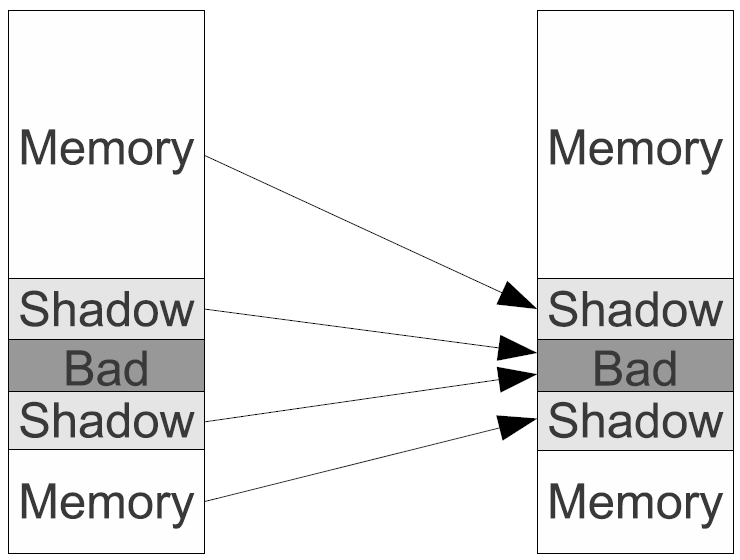
\includegraphics[width=0.4\textwidth]{img/shadow-memory.png}
  \caption{AddressSanitizer Speicherabbildung}
  \label{fig:shadow-memory}
\end{figure}

\subsection{Instrumentierung}

Die Instrumentierung geschieht am Ende der Optimierungspipeline des Compilers. 
Somit ist gewährleistet, dass nur diejenigen Speicherzugriffe instrumentiert
werden, die die Optimierung des Compilers überlebt haben. Die Funktion
\lstinline{ReportAndCrash(Addr)} wird an vielen Stellen im Code eingefügt, um
potentielle Speicherfehler zu melden.

Wenn ein 8-Byte-Speicherzugriff passieren soll, berechnet AddressSanitizer die
Adresse im \textit{Shadow Memory} nach der Formel, die in
~\cref{sec:asan-shadow-memory} erläutert wurde. Wie
in~\cref{lst:check-shadow-addr} zu erkennen ist, wird geprüft, ob der Inhalt
von \verb|ShadowAddr| ungleich $0$ ist. Ist das Shadow Byte ungleich null,
deutet dies darauf hin, dass der Speicherzugriff fehlerhaft ist.

\lstinputlisting[caption={Check ShadowAddr}, label={lst:check-shadow-addr}, language=C]{ressources/check-shadow-addr.c}

Für Speicherzugriffe mit weniger als 8 Bytes ist die Instrumentierung etwas
komplexer. Wenn das Shadow Byte positiv ist, wird überprüft, ob der Zugriff
innerhalb der erlaubten Grenzen liegt. \verb|AccessSize|
in~\cref{lst:check-shadow-addr-small-byte} ist die Größe des Speicherzugriffs
in Bytes.

\lstinputlisting[caption={Check ShadowAddr < 8 Byte}, label={lst:check-shadow-addr-small-byte}, language=C]{ressources/check-shadow-addr-small-byte.c}

\subsection{Laufzeitbibliothek}\label{sec:asan-runtime-lib}

Die Hauptaufgabe der Laufzeitbibliothek ist es, den \textit{Shadow Memory} zu
verwalten. Beim Start der Anwendung wird der gesamte Bereich des \textit{Shadow
  Memory} reserviert, sodass kein anderer Teil der Anwendung ihn nutzen kann.
Somit wird gewährleistet, dass der \textit{Shadow Memory} einzig für die
Überwachung des Anwendungsspeichers zur Verfügung steht.

Die Standardfunktionen \verb|malloc| und \verb|free| werden durch die
Laufzeitbibliothek überschrieben, um die Funktionalität des Konzepts hinter
AddressSanitizer sicherzustellen. Bei einer Speicherallokation wird eine
Speicherregion mit ihren Redzones vom Betriebssystem allokiert. Für $n$
Speicherregionen werden immer $n + 1$ Redzones allokiert, sodass die rechte
Redzone einer Speicherregion die linke Redzone einer anderen Speicherregion
ist. Redzone "`rz1"' in~\cref{tab:asan-memory-allocation} beinhaltet zusätzlich
Informationen des Allokators, wie zum Beispiel die Allokationsgröße, Thread-Id
usw.

\begin{table}[t]
  \caption{Laufzeitbibliothek Speicherallokation}
  \label{tab:asan-memory-allocation}
  \begin{tabular}{|
      >{\columncolor[HTML]{FE0000}}l |
      >{\columncolor[HTML]{C0C0C0}}l |
      >{\columncolor[HTML]{FE0000}}l |
      >{\columncolor[HTML]{C0C0C0}}l |
      >{\columncolor[HTML]{FE0000}}l |}
    \hline
    rz1 & mem1 & rz2 & mem2 & rz3 \\ \hline
  \end{tabular}
\end{table}

Die Speicherfreigbar mittels \verb|free| "`vergiftet"' den gesamten
Speicherbereich und legt ihn in Quarantäne, sodass er von \verb|malloc| nicht
erneut allokiert werden kann. Die Quarantäne wird als FIFO-Warteschlange
realisiert, die eine feste Menge an Speicher hält. Beide Speicherbefehle
(\verb|malloc| und \verb|free|) zeichnen den Callstack auf, um informative
Fehlerberichte liefern zu können.

\section{Technische Analyse: Memory Corruption Detector Sanitizer}

Im Paper \textit{Enhanced Memory Corruption Detection in C/C++
  Programs}~\cite{mcds_2023} stellen Ching-Yi Lin und Wuu Yang das neue Werkzeug
"`mcds"' vor und vergleichen es mit etablierten Tools wie zum Beispiel
AddressSanitizer. Die Speicherfehlererkennung ist Zeit- und Speicheraufwändig
und kann die Programmausführung erheblich verlangsamen. Hardwareunterstützung
könnte die Programmausführung beschleunigen, jedoch mangelt es an
Implementierungen, die diese Hardwareunterstützung
nutzen~\cite{hardware-asan_2024}.

Mit dieser Motivation wurde mcds entwickelt. Mcds nutzt die Intel
SGX-Erweiterungsunterstützung für hardwarebasiertes Shadow Memory. Mcds besteht
aus drei Teilen: Instrumentierung, einer Laufzeitbibliothek und Erweiterungen
mit Intel SGX.

Die Besonderheit von mcds ist, dass es Speicherfehler erkennt, die Redzones
fester Größe verursachen. Redzones fester Größe werden von vielen etablierten
Speicherfehlererkennungswerkzeugen wie auch AddressSanitizer verwendet.
In~\cref{fig:fixed-size-redzones} kann man einen solchen Speicherfehler sehen,
der bei AddressSanitizer nicht erkannt werden würde. Die Größe des Character
Arrays \lstinline{a} übersteigt die Größe von \lstinline{a} und seine Redzone.
Mcds erkennt Speicherfehler, die aus Redzones fester Größe resultieren dadurch,
dass mehrere virtuelle Speicherseiten in eine physikalische Speicherseite
zusammengefasst werden. Dadurch verursacht mcds keinen signifikanten
Speicherverbrauch und nutzt die Hardwarefähigkeiten für eine schnellere
Ausführung.

\begin{figure}[h]
  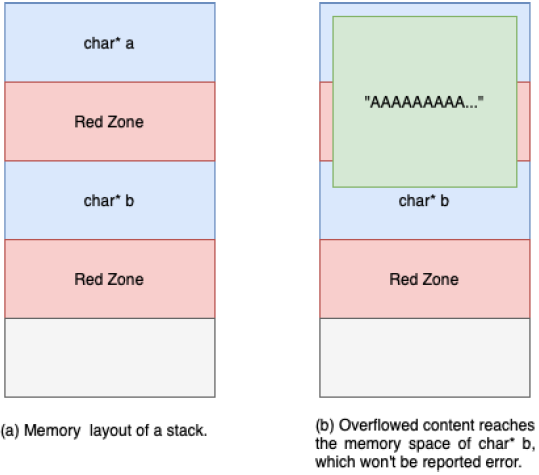
\includegraphics[width=0.4\textwidth]{img/fixed-size-redzone.png}
  \caption{Problem: Redzones fester Größe}
  \label{fig:fixed-size-redzones}
\end{figure}

\subsection{Instrumentierung}

Auch mcds macht von binärer Instrumentierung Gebrauch. Während der Kompilierung
wird ein "`Sanitizer Pass"' angewendet. Der Sanitizer Pass ist eine spezielle
Phase im Kompilierungsprozess, bei der der Code analysiert und modifiziert
wird. Der mcds-Sanitizer-Pass ersetzt dabei Aufrufe zur Speicherallokation und
Speicherfreigabe mit Aufrufen, die in der Laufzeitbibliothek von mcds definiert
sind. Zusätzlich wird eine Report-Funktion in die instrumentierte Binärdatei
eingefügt. Diese Funktion wird aufgerufen, wenn ein ungültiger Speicherzugriff
oder ein Prozessabsturz erkannt wird. Die Report-Funktion ist dafür
verantwortlich, detaillierte Fehlerberichte zu erstellen, die helfen, die
Quelle des Speicherfehlers zu identifizieren.

\subsection{Laufzeitbibliothek}

Die Laufzeitbibliothek von mcds beinhaltet den "`debug allocator"' und den
"`page fault analyzer"'. Der debug allocator verwaltet den Speicher, sodass
Speicherfehler gefunden werden können. Der page fault analyzer interpretiert
die Speicherseitenausnahmen.

Beim der Allokation von Speicher wird jedes Speicherobjekt auf eine separate
virtuelle Speicherseite abgebildet. So ist der Abstand zwischen einzelnen
(kleinen) Objekten im Speicher fast eine ganze Speicherseite. Um den
Speicherbedarf gering zu halten werden mehrere dieser virtuellen Speicherseiten
auf eine physikalische Speicherseite abgebildet. Dieser Vorgang wird
\textit{page aliasing} genannt~\cite{mcds_2023}.

Die Freigabe von Speicher wird die betroffene Speicherseite mit der
\verb|PROT_NONE| Flag ausgestattet. Die Seite wird zunächst unzugänglich für
andere Speicherzugriffe und wird geleert. Danach kommt die Seite wieder in den
Speicherpool zurück.

\subsection{Verwendung von Shadow Memory und Intel SGX}

Während Werkzeuge wie zum Beispiel AddressSanitizer softwarebasiertes
\textit{Shadow Memory} einsetzen, nutzt mcds Intel SGX (Software Guard
Extensions), um \textit{Shadow Memory} hardwareseitig zu implementieren. Dies
reduziert den Overhead, den es benötigt die Speicheradresse im \textit{Shadow
  Memory} zu berechnen. Auch wird Overhead minimiert, da die Redzones bei mcds
Seitenbasiert sind, während die Redzones bei AddressSanitizer nicht
zwangsläufig seitenbasiert ausgerichtet sind. Anstatt softwarebasiertes Shadow
Memory zu nutzen, um die Gültigkeit von Speicheradressen zu überprüfen,
verfolgt mcds die Signale des EPCM Registers. Diese Signale zeigen ungültige
Zugriffe an. Bei einem Verstoß gegen das EPCM Register wird ein Signal
ausgelöst, das vom Signal-Handler abgefangen wird, was eine effizientere
Fehlererkennung ermöglicht.

\section{Diskussion}

In diesem Kapitel sollen die beiden Speicherfehlererkennungswerkzeuge
AddressSanitizer und mcds miteinander verglichen werden. Dabei konzentrieren
wir uns auf Aspekte wie die Effizienz der Speicherverwaltung und die
Genauigkeit der Fehlererkennung.

AddressSanitizer, ein weit verbreitetes und anerkanntes Tool, verwendet eine
softwarebasierte Implementierung von Shadow Memory und Red Zones, um
Speicherfehler zu erkennen. Es nutzt Bit-Operationen, um die Zuordnung von
Speicheradressen zu überwachen und hat sich als effektiv erwiesen, bringt
jedoch einen signifikanten Zeit- und Speicheraufwand mit sich.

Mcds hingegen stellt eine neuere Lösung dar, die auf der LLVM-Toolchain basiert
und sich durch die Integration von Intel SGX (Software Guard Extensions)
auszeichnet. Diese Hardware-Unterstützung ermöglicht eine effizientere
Verwaltung des Shadow Memory, wodurch der Overhead reduziert und die Leistung
verbessert wird. Mcds verwendet seitenbasiert ausgerichtete Red Zones und nutzt
das Enclave Page Cache Map (EPCM) Register als Hardware-Shadow-Memory, was die
Fehlererkennung beschleunigt und die Robustheit erhöht, insbesondere in
Mehrprozess- und Multithread-Umgebungen.

Zuerst betrachten wir die Geschwindigkeit, bis ein Stack-Overflow-Fehler und
ein Use-After-Free-Fehler im Firefox-Projekt durch die beiden Werkzeuge
gefunden wurde. Dabei wurden dieselben Eingabemuster verwendet, um dieselben
Speicherfehler zu provozieren. Aus den Ergebnissen
aus~\cref{tab:firefox-error-speed} lässt sich schließen, dass mcds ungefähr 6
Mal schneller als AddressSanitizer ist. Die Spalte "`Core Dump"' gibt die
Ergebnisse für das Originalprogramm ohne Sanitizer an. Anhand der
Core-Dump-Ergebnisse und der mcds-Ergebnisse kann ein 2-facher Verlangsamung
durch die mcds-Erkennung angenommen werden. Ähnliche Ergebnisse lassen sich
auch aus~\cref{tab:chrome-error-speed} ableiten. Dort wurden ebenfalls
AddressSanitizer und mcds verglichen, wie sie beim Chrome Browser Projekt
abschneiden. Die Core Dump Spalte zeigt ebenfalls die Zeit zum Absturz ohne
Speicherfehlererkennungswerkzeug.

\begin{table}[]
  \caption{Geschwindigkeitsvergleich beider Werkzeuge Firefox}
  \label{tab:firefox-error-speed}
  \begin{tabular}{l|lll}
                   & AddressSanitizer & mcds   & Core Dump \\ \hline
    Stack Overflow & 532,1 s          & 97,3 s & 42,3 s    \\
    Use-After-Free & 627,5 s          & 103,4  & 52,7 s
  \end{tabular}
\end{table}

\begin{table}[]
  \caption{Geschwindigkeitsvergleich beider Werkzeuge Chrome}
  \label{tab:chrome-error-speed}
  \begin{tabular}{l|lll}
                   & AddressSanitizer & mcds    & Core Dump \\ \hline
    Stack Overflow & 631,85 s         & 51,64 s & 32,14 s   \\
    Use-After-Free & 985,1 s          & 86,02 s & 47,34 s
  \end{tabular}
\end{table}

Durch die Implementierung der binären Instrumentierung verlängern sich auch die
Kompilierzeiten der Software, die mit einem Speicherfehlererkennungswerkzeug
ausgestattet wird. Aus~\cref{tab:compile-time} lassen sich die Kompilierzeiten
von Firefox, Chrome und PHP ablesen. Die Projekte wurden jeweils mit
AddressSanitizer und mcds ausgestattet, sowie ohne
Speicherfehlererkennungswerkzeug kompiliert. Die Messergebnisse zeigen, dass
sich keine signifikante Zeitunterschiede zwischen den beiden Werkzeugen
ergeben. Das Ausstatten der Softwareprojekte mit einem der beiden Werkzeuge
resultiert in einer Verdoppelung der Kompilierzeit.

\begin{table}[]
  \caption{Kompolierzeiten einzelner Projekte}
  \label{tab:compile-time}
  \begin{tabular}{l|lll}
            & AddressSanitizer & mcds         & Ohne Werkzeug \\ \hline
    Firefox & 2h 56min 5s      & 2h 15min 17s & 1h 23min 10s  \\
    Chrome  & 2h 13min 3s      & 2h 24min 23s & 1h 10min 7s   \\
    PHP     & 8h 42min 2s      & 9h 2min 4s   & 4h 27min 12s
  \end{tabular}
\end{table}

\section{Verwandte Arbeiten}

Die in den Arbeiten genannten Referenzen sind essentiel, um den erweiterten
Kontext der beiden Werkzeuge zu verstehen. Zum einen finden wir dort
Dokumentation zu Werkzeugen, die mit AddressSanitizer oder mcds verglichen
werden. Auch in dieser Arbeit sind Dokumentation zu anderen Werkzeugen, wie zum
Beispiel Apples Malloc Debugging Feature~\cite{guard-malloc_2024}, aufgelistet.
Die referenzierten Arbeiten stellen nicht nur Begriffserklärungen bereit,
sondern helfen auch die wissenschaftlichen Erkenntnisse der Arbeiten in einen
zeitlichen und wissenschaftlichen Rahmen einzuordnen.

Begriffserklärungen finden wir in dieser Arbeit zum Beispiel in \textit{Modern operating Systems} von Tanenbaum und Bos~\cite{tanenbaum-modern_2015}, welches ein Standardwerk zu modernen
Betriebssystemen ist. Bei AddressSanitizer und mcds lässt sich gut erkennen,
dass dort viele Quellen zu Referenzimplementierung genannt sind. Somit lässt
sich die Lösung mit anderen Lösungen vergleichen und Vor- und Nachteile
gegenüberstellen.

\section{Schluss}

In dieser Arbeit wurden die Werkzeuge AddressSanitizer und mcds
detailliert untersucht und verglichen, wobei deren Ansätze zur Erkennung und
Vermeidung von Speicherfehlern im Vordergrund standen. Beide Werkzeuge haben
sich als leistungsfähige Lösungen zur Verbesserung der Software-Sicherheit
erwiesen, jedoch mit unterschiedlichen Stärken und Schwächen.

AddressSanitizer ist ein etablierter Ansatz zur Erkennung von Speicherfehlern,
der durch seine umfassende Unterstützung und Integration in Compiler-Frameworks
wie LLVM weit verbreitet ist. Im Gegensatz dazu nutzt mcds einen innovativen
Ansatz, der hardwaregestützte Techniken wie Intel SGX integriert, um die
Effizienz der Speicherüberwachung zu verbessern. Durch die Nutzung von
seitenbasierten Red Zones und die Verwendung von Hardwareunterstützung zur
Validierung von Speicherzugriffen kann mcds den Laufzeit-Overhead signifikant
reduzieren. Dies macht mcds besonders geeignet für Anwendungen, die eine hohe
Leistung erfordern und gleichzeitig gegen Speicherfehler geschützt werden
müssen. Die Ergebnisse der durchgeführten Experimente zeigen, dass mcds in
vielen Szenarien schneller arbeitet als AddressSanitizer, insbesondere bei der Erkennung
temporaler Speicherfehler.

Insgesamt bieten beide Werkzeuge wertvolle Beiträge zur Verbesserung der
Software-Sicherheit. Zukünftige Arbeiten könnten darauf abzielen, die Vorteile
beider Ansätze zu kombinieren und die Hard- und Softwarekombination, die durch
mcds eingeführt wurde, zu optimieren oder dessen Komplexität zu reduzieren. Die
kontinuierliche Weiterentwicklung und Verfeinerung von Werkzeugen wie AddressSanitizer und
mcds wird entscheidend dazu beitragen, die Zuverlässigkeit und Sicherheit
moderner Softwareanwendungen zu erhöhen.

%% The next two lines define the bibliography style to be used, and
%% the bibliography file.
\bibliographystyle{ACM-Reference-Format}
\bibliography{AutomatisierteSpeicherfehlererkennung/bib}

\end{document}
\endinput
%%
%% End of file `sample-acmtog.tex'.
